\chapter{فرز الكائنات الحية}\label{ch:g3:sorting-living-things}

اقلب علبة أزرار مختلطة على الطاولة، فتبدأ يداك \omterm{def:g3:sorting-living-things:criterion}{الفرز} من تلقاء
نفسيهما: الكبير مع الكبير، والأحمر مع الأحمر، وذو الأربعة ثقوب مع
مثله. وقد أحسّ علماء الطبيعة بالدافع نفسه أمام خليط العالم الحي من
الخنافس \omterm{prop:g3:sorting-living-things:groups}{والطيور} والسرخسيات \omterm{prop:g3:sorting-living-things:groups}{والأسماك} --- وتبين أن \omterm{def:g3:sorting-living-things:criterion}{فرز} الكائنات
الحية بعناية من أقوى أفكار \omterm{def:g1:living-or-not:living}{علم الأحياء}.

\section{الفرز يحتاج إلى قاعدة}

\begin{definition}[الفرز والمحكّات]\label{def:g3:sorting-living-things:criterion}
أن \emph{تفرز}\index{فرز} مجموعة هو أن تجمع ما يتفق منها معًا.
و\emph{المحكّ}\index{محك} هو القاعدة المستعملة في الفرز --- ``له
ست \omterm{def:g1:my-body:parts}{أرجل}''، ``له \omterm{def:g1:animals-around-us:covering}{ريش}''. والمحكّ الجيد للكائنات الحية صفة في الجسم
تستطيع \emph{ملاحظتها}: شيء \emph{يملكه} \omterm{def:g1:animals-around-us:animal}{الحيوان} أو \omterm{def:g1:plants-around-us:plant}{النبات}، لا
المكان الذي يعيش فيه ولا ما يصادف أن يفعله.
\end{definition}

\begin{example}[فرزان للحيوانات نفسها]\label{ex:g3:sorting-living-things:two}
خذ القطة والبطة والسلمون المرقط والدعسوقة. فبمحكّ ``يعيش قرب
الماء'' تجتمع البطة والسلمون. وبمحكّ ``له \omterm{def:g1:animals-around-us:covering}{ريش}'' تقف البطة وحدها.
وكلاهما \omterm{def:g3:sorting-living-things:criterion}{فرز} --- لكن الثاني وحده يستعمل جسم \omterm{def:g1:animals-around-us:animal}{الحيوان} نفسه، وهو الصنف
الذي يثق به علماء الأحياء: \omterm{def:g1:animals-around-us:animal}{فالحيوان} يستطيع أن ينتقل من بيت إلى
بيت، لكنه لا يستطيع أن يبدّل ريشه بحراشف.
\end{example}

\begin{remark}[لماذا لا نفرز بالبيت أو المائدة؟]\label{rem:g3:sorting-living-things:why}
\omterm{def:g2:where-animals-live:habitat}{الموئل} والمائدة يتغيران بتغير فصول السنة وبالحظ --- فشحرور
\cref{ch:g2:what-animals-eat} ينتقل من الديدان إلى التوت من غير أن
يصير حيوانًا آخر. أما صفات الجسم فتبقى. ولهذا يغلب ``ما يملكه'' على
``ما يفعله'' قاعدةً \omterm{def:g3:sorting-living-things:criterion}{للفرز}.
\end{remark}

\section{مجموعات الحيوانات الكبرى}

\begin{proposition}[بعض المجموعات الكبرى]\label{prop:g3:sorting-living-things:groups}
\omterm{def:g3:sorting-living-things:criterion}{الفرز} بصفات الجسم يجمع \omterm{def:g1:animals-around-us:animal}{الحيوانات} في مجموعات كبرى، منها:
\begin{itemize}
  \item \emph{الحشرات}\index{حشرة}: ست \omterm{def:g1:my-body:parts}{أرجل}، وجسم من ثلاثة أقسام
        --- كالنملة والدعسوقة والنحلة والفراشة؛
  \item و\emph{الأسماك}\index{سمكة}: زعانف وحراشف، وحياة تقضى في
        الماء --- كالسلمون المرقط والسمكة الذهبية؛
  \item و\emph{الطيور}\index{طائر}: \omterm{def:g1:animals-around-us:covering}{ريش} وأجنحة ومنقار --- كالبطة
        والشحرور والنعامة؛
  \item و\emph{الثدييات}\index{ثديي}: \omterm{def:g1:animals-around-us:covering}{فرو} أو شعر، وأمهات تُرضع
        صغارها \omterm{def:g2:animals-grow-up:born}{الحليب} --- كالقطة والبقرة والخفاش والحوت ---
        والبشر؛
  \item و\emph{البرمائيات}\index{برمائي}: \omterm{def:g1:the-five-senses:sense}{جلد} رطب، \omterm{def:g2:animals-grow-up:born}{وبيض} يوضع في
        الماء، وطفولة شرغوفية --- كالضفدع والسمندل.
\end{itemize}
\end{proposition}
\admitted

\begin{omfigure}
\begin{tikzpicture}
  \foreach \x/\name/\feat in {
      0/حشرات/{6 أرجل},
      2.95/أسماك/{زعانف وحراشف},
      5.9/طيور/{ريش ومنقار},
      8.85/ثدييات/{فرو وحليب},
      11.8/برمائيات/{جلد رطب}} {
    \draw[thick, omDef, fill=omDef!6, rounded corners=5pt]
      (\x,0) rectangle ({\x+2.8},1.7);
    \node[font=\small\bfseries, text height=1.6ex, text depth=0.4ex]
      at ({\x+1.4},1.3) {\name};
    \node[font=\small, text height=1.6ex, text depth=0.4ex]
      at ({\x+1.4},0.6) {\feat};
  }
\end{tikzpicture}

{\small خمس مجموعات كبرى، كل واحدة مسماة بما \emph{تملكه}.}
\end{omfigure}

\begin{example}[مفاجآت على وجهها الصحيح]\label{ex:g3:sorting-living-things:surprises}
المحكّات تنقذنا من التخمينات الكسولة. فالخفاش يطير كالطائر ---
لكن له فروًا لا ريشًا، وهو يُرضع صغاره \omterm{def:g2:animals-grow-up:born}{الحليب}: إنه من \omterm{prop:g3:sorting-living-things:groups}{الثدييات}.
والحوت يسبح كالسمكة --- وفروه تضاءل حتى كاد يزول، لكنه يُرضع عجله
\omterm{def:g2:animals-grow-up:born}{الحليب} ولا حراشف له: من \omterm{prop:g3:sorting-living-things:groups}{الثدييات} أيضًا. والنعامة لا تطير البتة،
ومع ذلك يقول \omterm{def:g1:animals-around-us:covering}{الريش} والمنقار: طائر. \omterm{def:g3:sorting-living-things:criterion}{فالمحكّ} هو الذي يقرر، لا
الانطباع.
\end{example}

\begin{omfigure}
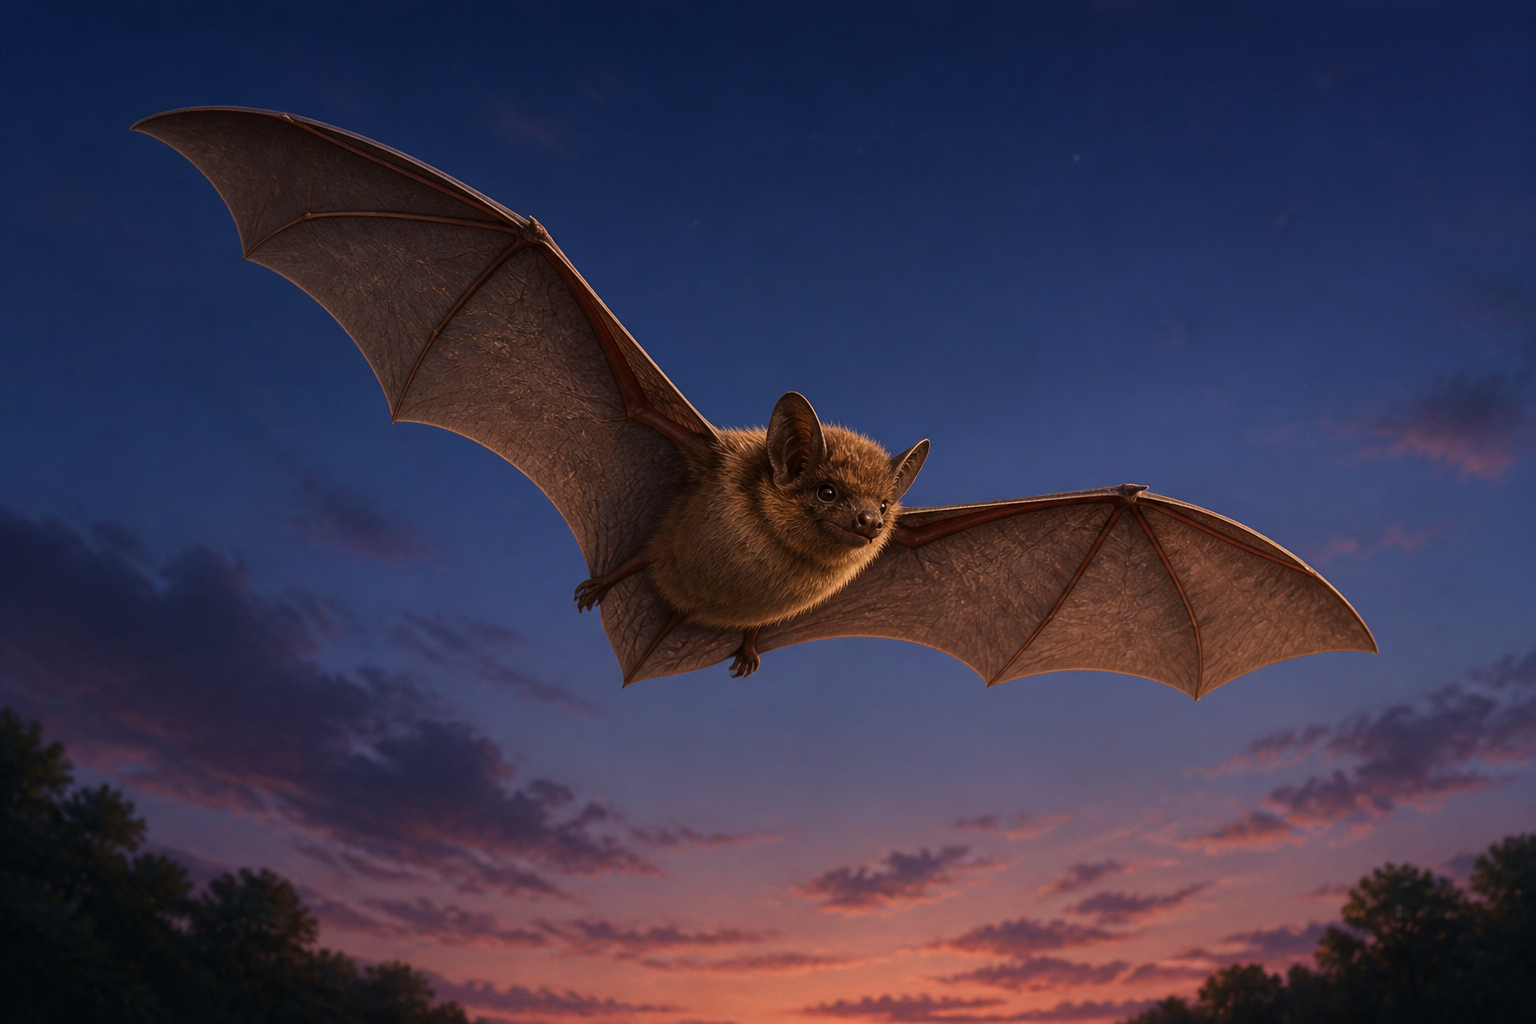
\includegraphics[width=0.6\linewidth]{images/book1/ai/g3-sort-bat.png}

{\small يطير كالطائر --- ويلبس فروًا على جناحين عاريين: الخفاش،
الاختبار الكلاسيكي \omterm{def:g3:sorting-living-things:criterion}{للفرز} بالصفات لا بالانطباعات.}
\end{omfigure}

\begin{method}[فرز حيوان مجهول]\label{met:g3:sorting-living-things:sort}
\begin{enumerate}
  \item لاحظ الجسم: أجلد أم \omterm{def:g1:animals-around-us:covering}{فرو} أم \omterm{def:g1:animals-around-us:covering}{ريش} أم حراشف؟ وكم رجلًا؟ وأله
        أجنحة؟ وأله منقار؟
  \item واسأل عن الصغار إن استطعت: أحليب؟ أم \omterm{def:g2:animals-grow-up:born}{بيض}؟ أم مرحلة
        شرغوف؟
  \item وقارن بمجموعات \cref{prop:g3:sorting-living-things:groups}
        وضع \omterm{def:g1:animals-around-us:animal}{الحيوان} حيث تناسب \emph{صفاته}؛
  \item وإن خالف انطباعٌ (``إنه يطير!'') صفةً (``له \omterm{def:g1:animals-around-us:covering}{فرو}'')، فثق
        بالصفة.
\end{enumerate}
\end{method}

\section{النباتات تُفرز أيضًا}

\begin{proposition}[فرز النباتات]\label{prop:g3:sorting-living-things:plants}
تُفرز \omterm{def:g1:plants-around-us:plant}{النباتات} بصفاتها كما تُفرز \omterm{def:g1:animals-around-us:animal}{الحيوانات}. ومن المحكّات المفيدة:
أيصنع \emph{أزهارًا} وبذورًا (كالأقحوان والكستناء) أم لا يصنعها
البتة (كالسرخس والطحلب)؟ وأساقه طرية خضراء أم خشبية كجذع
\emph{الشجرة}؟ وأأوراقه عريضة أم إبر كإبر الصنوبر؟
\end{proposition}
\admitted

\begin{example}[ثلاثة أركان من المتنزه]\label{ex:g3:sorting-living-things:park}
في متنزه واحد: شجيرة الورد --- أزهار \omterm{def:g1:plants-around-us:parts}{وسيقان} خشبية؛ والطحلب على
الجدار الشمالي --- لا أزهار له البتة ولا \omterm{def:g1:plants-around-us:parts}{ساق} حقيقية؛ والصنوبرة ---
شجرة ذات إبر وأكواز. ثلاثة \omterm{def:g1:plants-around-us:plant}{نباتات}، وثلاثة أجوبة مختلفة عن
المحكّات نفسها.
\end{example}

\begin{remark}[الفرز أول خطوة في علم]\label{rem:g3:sorting-living-things:science}
المجموعات المفروزة جيدًا تتيح للناس أن يسألوا أسئلة أفضل: فما يصح
على \omterm{prop:g3:sorting-living-things:groups}{الحشرات} عمومًا --- ست \omterm{def:g1:my-body:parts}{أرجل}، وجسم من ثلاثة أقسام، وأجنحة في
الغالب --- يصير معروفًا فجأة لمئات آلاف الأنواع دفعةً واحدة.
وستحوّل فصول لاحقة \omterm{def:g3:sorting-living-things:criterion}{الفرز} إلى شجرة نسب لكل الكائنات الحية ---
والآن تعلّم أن \omterm{def:g3:sorting-living-things:criterion}{تفرز} بما تستطيع رؤيته.
\end{remark}

\section{تمارين}

\begin{exercise}[$\star$]\label{exo:g3:sorting-living-things:1}
ما \omterm{def:g3:sorting-living-things:criterion}{المحكّ}؟ أعطِ محكًّا جيدًا \omterm{def:g3:sorting-living-things:criterion}{لفرز} \omterm{def:g1:animals-around-us:animal}{الحيوانات}، ومحكًّا يتجنبه علماء
الأحياء.
\end{exercise}

\begin{exercise}[$\star$]\label{exo:g3:sorting-living-things:2}
أعطِ الصفة (أو الصفات) التي تحدّ كل مجموعة: \omterm{prop:g3:sorting-living-things:groups}{الحشرات}، \omterm{prop:g3:sorting-living-things:groups}{والأسماك}،
\omterm{prop:g3:sorting-living-things:groups}{والطيور}، \omterm{prop:g3:sorting-living-things:groups}{والثدييات}.
\end{exercise}

\begin{exercise}[$\star$]\label{exo:g3:sorting-living-things:3}
ضع كل \omterm{def:g1:animals-around-us:animal}{حيوان} في مجموعته: النحلة، والسمكة الذهبية، والنعامة،
والبقرة، والضفدع.
\end{exercise}

\begin{exercise}[$\star$]\label{exo:g3:sorting-living-things:4}
الخفاش يطير. فلماذا كان من \omterm{prop:g3:sorting-living-things:groups}{الثدييات} لا من \omterm{prop:g3:sorting-living-things:groups}{الطيور}؟ وأي الصفات
تقرر؟
\end{exercise}

\begin{exercise}[$\star$]\label{exo:g3:sorting-living-things:5}
الحوت يعيش في البحر. فلماذا لم يكن سمكة؟ وأي الصفات تقرر؟
\end{exercise}

\begin{exercise}[$\star$]\label{exo:g3:sorting-living-things:6}
للعنكبوت ثماني \omterm{def:g1:my-body:parts}{أرجل}. أيمكن أن يكون حشرة؟ وبم يجيب \omterm{def:g3:sorting-living-things:criterion}{المحكّ}؟
\end{exercise}

\begin{exercise}[$\star$]\label{exo:g3:sorting-living-things:7}
افرز هذه \omterm{def:g1:plants-around-us:plant}{النباتات} بمحكّات \cref{prop:g3:sorting-living-things:plants}:
الأقحوان، والطحلب، والصنوبر، وشجيرة الورد.
\end{exercise}

\begin{exercise}[$\star$]\label{exo:g3:sorting-living-things:8}
جرّب: افرز \omterm{def:g1:animals-around-us:animal}{حيوانات} شارعك أو حديقتك --- كل ما تستطيع رصده في نزهة
--- في مجموعات هذا الفصل. أي مجموعة تفوز عددًا؟
\end{exercise}

\begin{exercise}[$\star\star$]\label{exo:g3:sorting-living-things:9}
\omterm{def:g3:sorting-living-things:criterion}{تفرز} ليا \omterm{def:g1:animals-around-us:animal}{الحيوانات} إلى ``أليفة'' و``برية''. \omterm{def:g3:sorting-living-things:criterion}{وتفرز} صديقتها
\omterm{def:g1:animals-around-us:animal}{الحيوانات} نفسها إلى ``ثدييات'' و``طيور''. أي الفرزين \omterm{def:g3:sorting-living-things:criterion}{فرز} عالم
الأحياء، ولماذا؟ استعمل \cref{rem:g3:sorting-living-things:why}.
\end{exercise}

\begin{exercise}[$\star\star$]\label{exo:g3:sorting-living-things:10}
البطريق يسبح إتقانًا، ولا يستطيع الطيران، وهو مكسو بما يشبه
القرميد اللامع. فينظر عالم طبيعة عن قرب: ``القرميد'' \omterm{def:g1:animals-around-us:covering}{ريش} متراصّ،
وثمة منقار. طبّق \cref{met:g3:sorting-living-things:sort} على
البطريق، خطوةً خطوة.
\end{exercise}
